\subsection{Problem Definition}
\label{sec:problem}

%Next, we introduce notation and definitions used in our approach, and we formally define the problem addressed in this paper.

%\subsection{Geolocated Time Series}
%\label{subsec:preliminaries}

A {\em time series} is a time-ordered sequence of values $T = \{v_1, \ldots, v_n\}$, where $v_i$ is the value at the $i$-th time point and $n$ is the length of the series. Typically, as absolute values are usually less informative compared to the trends in a sequence, a $z$-{\em normalization} of the amplitudes is applied \cite{DBLP:conf/cp/GoldinK95}, so that the transformed time series approximately follow a standard Gaussian distribution $\mathcal{N}(0,1)$. We assume that this is done in a preprocessing step, applied similarly over all time series in a given dataset $\mathcal{T}$. As in other prior works like \cite{shieh2008kdd}, we use the Euclidean distance to measure the {\em similarity} between a pair of time series $T$ and $T'$ of equal length $n$:
\begin{equation} \label{eq:dist_ts}
d_{ts}(T, T') = \sqrt{\displaystyle \sum_{i=1}^{n}(T.v_i - T'.v_i)^2}.
\end{equation}

In this work, we specifically deal with time series that are additionally characterized by a \emph{location}, denoted by $T.loc$. In the sequel, when it is clear from the context, we also refer to such geolocated time series as objects for brevity.  Assuming a 2-dimensional space, we further use the notation $T.loc_x$, $T.loc_y$ to refer to the $(x,y)$ coordinates of $T$'s location. In the {\em spatial domain}, the {\em proximity} between two geolocated time series $T$ and $T'$ is calculated using the Euclidean distance of their respective locations:
\begin{equation} \label{eq:dist_sp2}
d_{sp}(T, T') = \sqrt{(T.loc_x - T'.loc_x)^2 + (T.loc_y - T'.loc_y)^2}.
\end{equation}

%%%%%%%%%%%%%%%%%%%%%%%%%
\eat{
In the {\em spatial domain}, the distance between two geolocated time series $T$ and $T'$ is calculated according to the {\em infinity norm (Chebyshev) distance} $L_{\infty}$, so it provides the greatest of their absolute difference in coordinate values along either dimension:
\begin{equation} \label{eq:dist_sp}
d_{sp}(T, T') = \max ( |T.loc_x - T'.loc_x| , |T.loc_y - T'.loc_y| ).
\end{equation}
}
%%%%%%%%%%%%%%%%%%%%%%%%%


%Note that in either domain, we may use other suitable similarity metrics, not only between locations, but also over time series, even complex measures as in \cite{paparrizos2015k}. Specification of a different distance measure can be trivially accommodated in our methodology.


%%%%%%%%%%%%%%%%%%%%%%%%%
\eat{
Without loss of generality, in the {\em time series domain} we assume that objects $T$ and $T'$ under comparison have equal length $n$. In this case, we measure their absolute difference at each time point and take the maximum of these deviations as the measure of their similarity: 
\begin{equation} \label{eq:dist_ts}
d_{ts}(T, T') =  \max ( \{ |T.v_i - T'.v_i | : i = 1..n \} ).
\end{equation}
Note that distance $d_{ts}$ in Eq.~\ref{eq:dist_ts} is an upper bound to the corresponding Euclidean distance over the same time series.
}
%%%%%%%%%%%%%%%%%%%%%%%%%


%\checknote{In case of time series with different lengths, we consider that $d_{ts}(T, T') = \infty$, because at certain time points the deviation between values cannot be calculated.}

%\subsection{Hybrid Similarity Joins over Geolocated Time Series}
%\label{subsec:sim_joins}

We can now formally introduce our problem: 

\begin{mydefinition}[Hybrid Similarity Join over Geolocated Time Series]\label{def:sim_join}
	Given two sets of geolocated times series $\mathcal{T}_{R}$ and $\mathcal{T}_{S}$, and two thresholds $\epsilon_{sp}$ and $\epsilon_{ts}$, the {\em hybrid similarity join} query returns all pairs qualifying w.r.t. to both criteria on spatial proximity and time series similarity, i.e., 
	\[ \{ (T_{R}, T_{S}): T_{R} \in \mathcal{T}_{R}, T_{S} \in \mathcal{T}_{S}, d_{sp}(T_{R}, T_{S})\leq\epsilon_{sp} \land d_{ts}(T_{R}, T_{S}) \leq \epsilon_{ts} \}. \] 
	%\qed
\end{mydefinition} 

%\begin{mydef}[Hybrid Similarity Join Queries over Geolocated Time Series]\label{def:sim_join}
%Given a query $q$ specifying a spatial distance radius $\epsilon_{sp}$, and a maximum deviation $\epsilon_{ts}$ in time series values over two datasets $\mathcal{T}_{R}, \mathcal{T}_{S}$ of geolocated time series, their {\em similarity join} provides all pairs qualifying w.r.t. to both criteria on spatial proximilty and time series similarity, i.e., 
%\[ \{ (T_{R}, T_{S}): T_{R} \in \mathcal{T}_{R}, T_{S} \in \mathcal{T}_{S}, d_{sp}(T_{R}, T_{S})\leq\epsilon_{sp} \land d_{ts}(T_{R}, T_{S}) \leq \epsilon_{ts} \}. \] 
%%\qed
%\end{mydef} 
 
That is, this query searches for pairs of objects that are within spatial distance at most $\epsilon_{sp}$, while also their respective time series do not deviate by more than~$\epsilon_{ts}$. Spatial proximity is measured in distance units (e.g., meters). As mentioned before, since the (transformed) time series are $z$-normalized, values for parameter $\epsilon_{ts}$ are {\em unitless} and are typically expressed in standard deviations.
  
\begin{myexample}
Figure~\ref{fig:simjoin_example} depicts two sets of geolocated time series, $\{R_1, \dots, R_5\}$ (in red bullets) and $\{S_1, \dots, S_6\}$ (in green squares) that represent CO$_2$ emissions collected by two sensor networks $R$ and $S$ in an urban area during a day. Suppose that a similarity join query over those two datasets specifies a distance radius $\epsilon_{sp} = 500$ meters to identify nearby sensors and a maximum deviation of $\epsilon_{ts} = 0.4$ to find similar CO$_2$ patterns. Qualifying pairs  $\{ (R_1, S_5), (R_3, S_5),  (R_5, S_2) \}$ are shown connected with dashed lines. Note that other pairs, e.g., $(R_4, S_3)$, may be even closer in space, but their time series deviate more than the given $\epsilon_{ts}$, so they are filtered out. Besides, time series like those in rejected pair $(R_3, S_3)$ may have almost the same pattern, but their locations are too far from each other to qualify for this query.
\qed
\end{myexample}

\begin{figure}[!t]
 \centering
{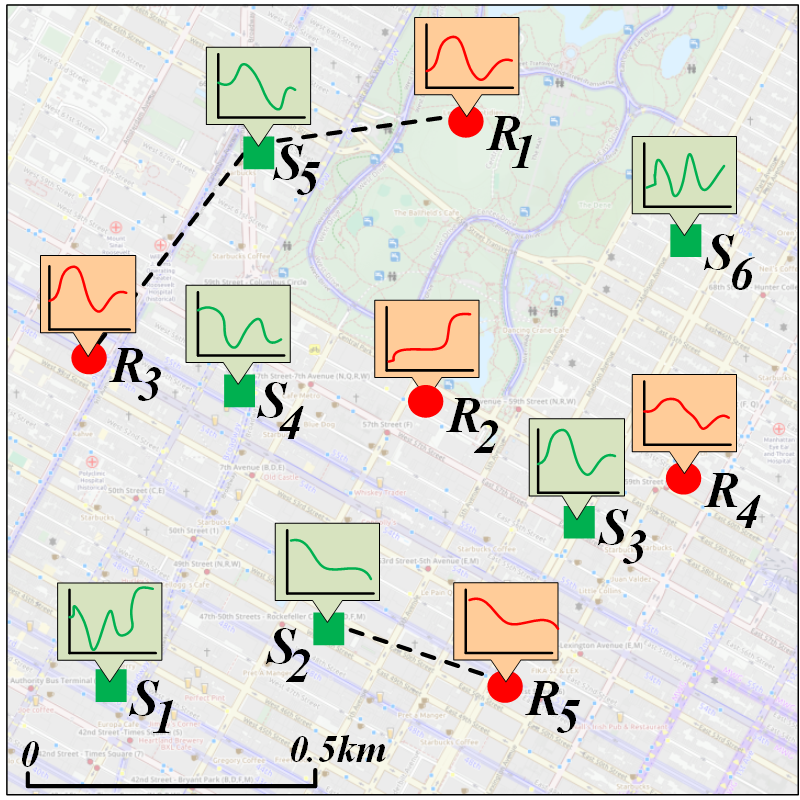
\includegraphics[width=0.28\textwidth]{figures/sim_join.png}}
 \vspace{-10pt}
\caption{Hybrid similarity join over geolocated time series.}
\label{fig:simjoin_example}
\end{figure}